

%%%%%%%%%%%%%%%%%%%%%%%%%%%%%%%%%%%%%%%%%%%%%%%%%%%%%%%%%%%%%%%%%%%%%%%%%%%%%%
\section{Run 105038 : regular mode }

\subsection{Time distribution and occupancy}
In run 105038, the length of the event window was reduced to 25 us,
the rate of the FPGA internal pulsers was kept at 60 khZ. 

Similar to \del{the approach outlined in} Section \ref{over}, Figure \ref{fig:4} shows the \del{first} distribution
\del{to watch was the time distribution} of the number of hits in two channels, one from the \del{channels of the}
first and \add{another one - from the} second FPGA. 
\del{Given that we are not operating in an overflow mode, our observations 
  reveal a uniform temporal distribution for both cases, as we expected.
}
\add{
  In this readout configuration, the expected number of pulses in a given channel
  within the event window is one or two, and the total number of pulses is always below 255.
}
\begin{figure}[H]
  \hspace{-0.5in}
  \begin{tikzpicture}
    \node[anchor=south west,inner sep=0] at (0,0.) {
      % \node[shift={(0 cm,0.cm)},inner sep=0,rotate={90}] at (0,0) {}
      % \makebox[\textwidth][c] {
      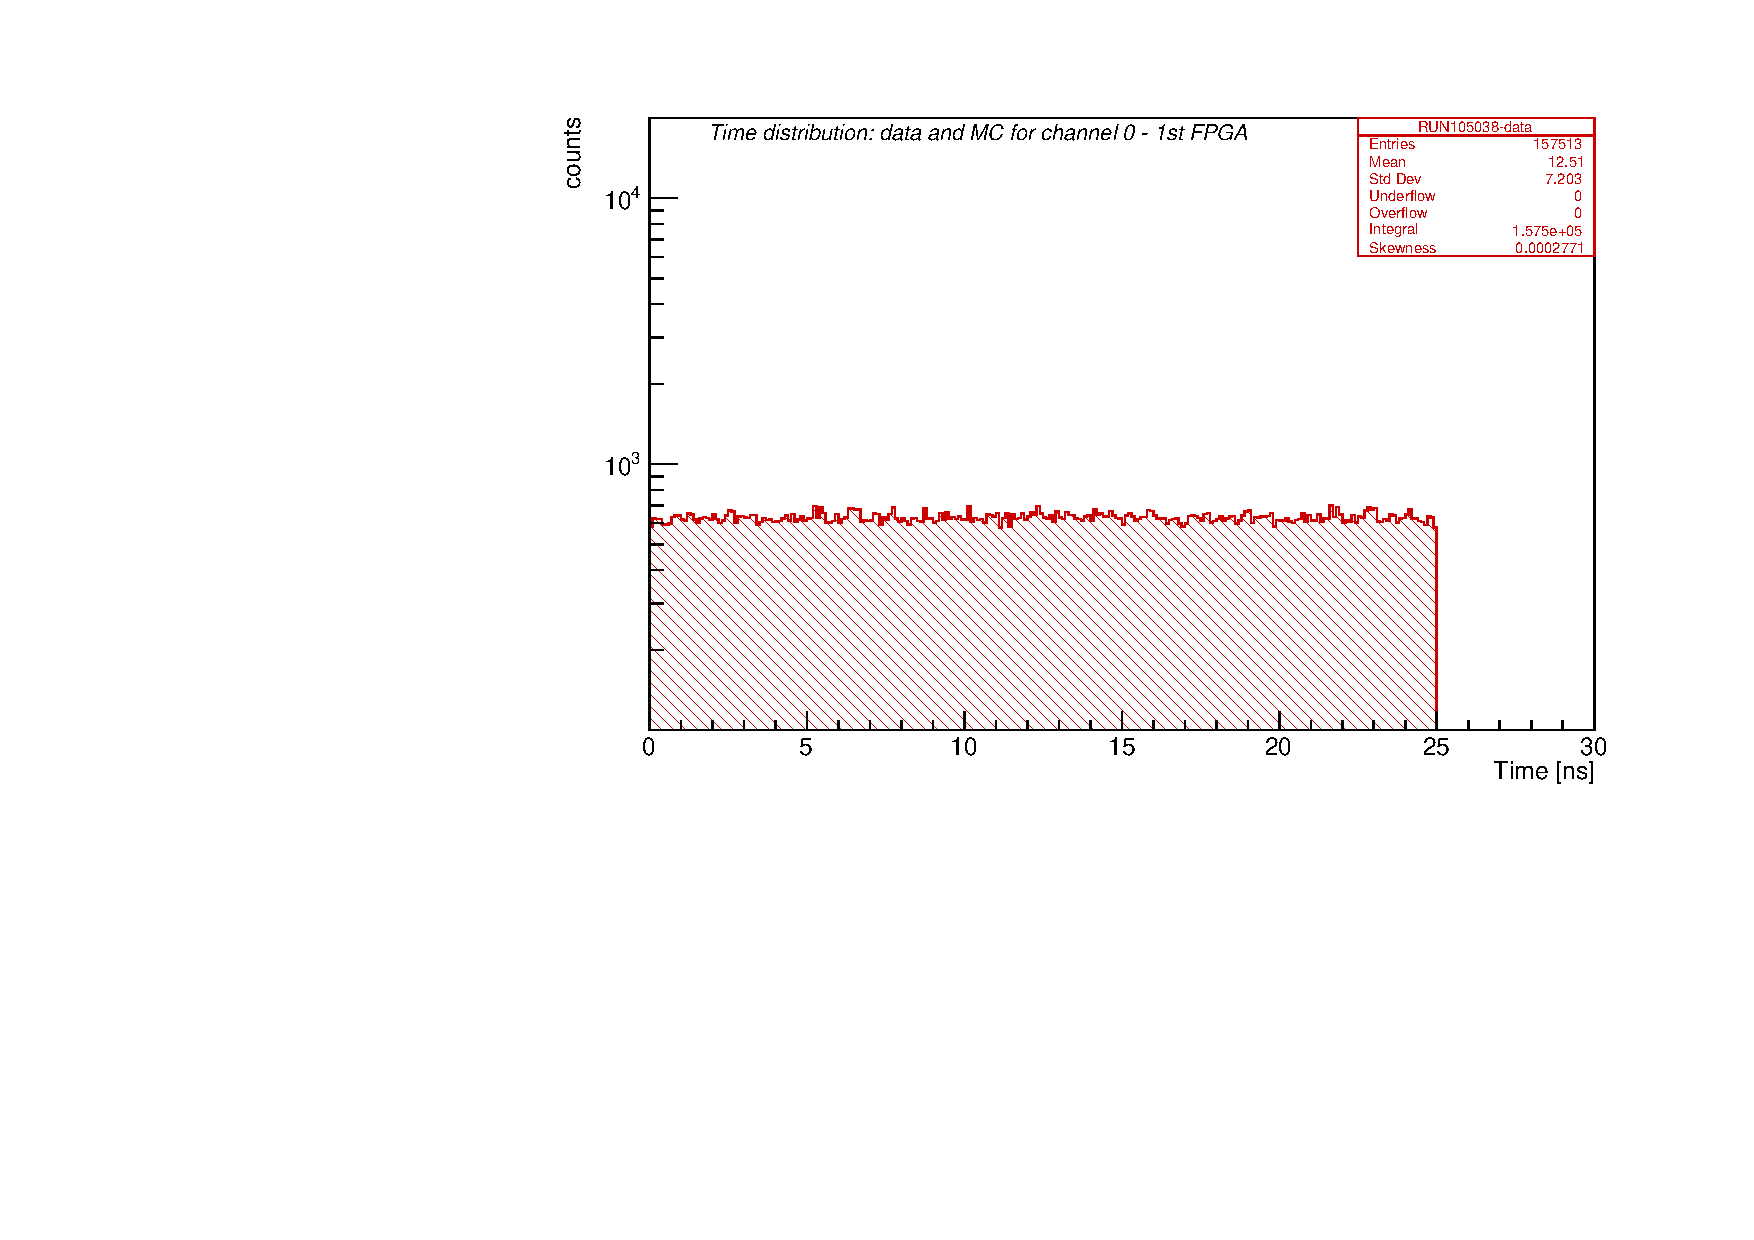
\includegraphics[width=0.5\textwidth]{figures/pdf/figure_00001_timedistr_roc_simulation_10538}
      % }
    };
    \node[anchor=south west,inner sep=0] at (10,0.) {
      % \node[shift={(0 cm,0.cm)},inner sep=0,rotate={90}] at (0,0) {}
      % \makebox[\textwidth][c] {
      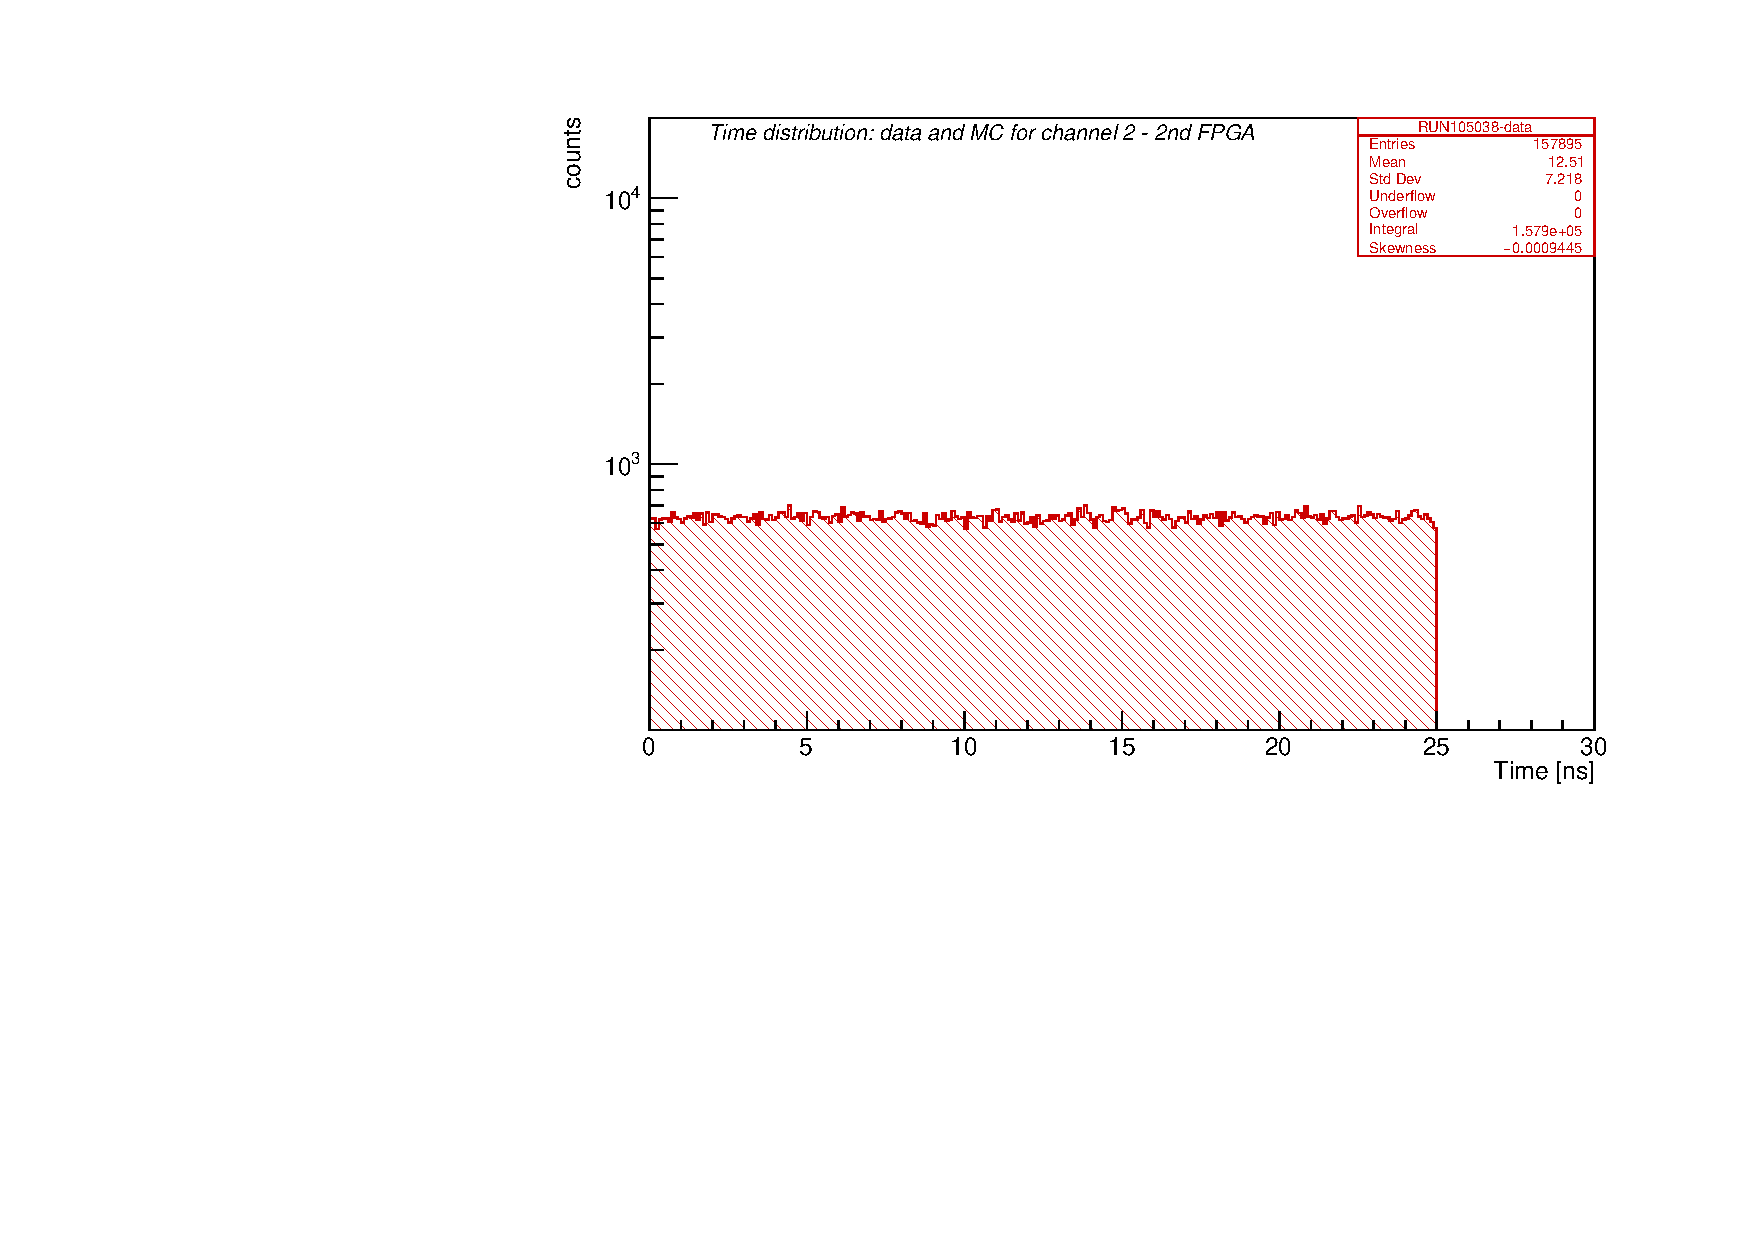
\includegraphics[width=0.5\textwidth]{figures/pdf/figure_00012_timedistr_roc_simulation_ch2_105038}
      % }
    };
  \end{tikzpicture}
  \caption{
    \label{fig:4}
    \del{right: First FPGA's channel time distribution, left: Second FPGA's channel time distribution.}
    \add{
      right: the hit time distribution for hits in channel 0, the first FPGA;
      left: the hit time distribution for htis in channel 2, the second FPGA.
    }
  }
\end{figure}
\add{
  In this mode, the readout of a given channel is not affected by the readout of previous
  channels and the ``occupancy'' distributions shown in Figure \ref{fig:5} are, as expected, uniform.
  }
\del{
  The time distibution can be easily understood by watching the occupancy plot in Fig.\ref{fig:5}.
  The occupancy is a uniform distribution, as we expected operating in a non-overflow mode. Channels ordering is the readout order.
}
\begin{figure}[H]
\centering
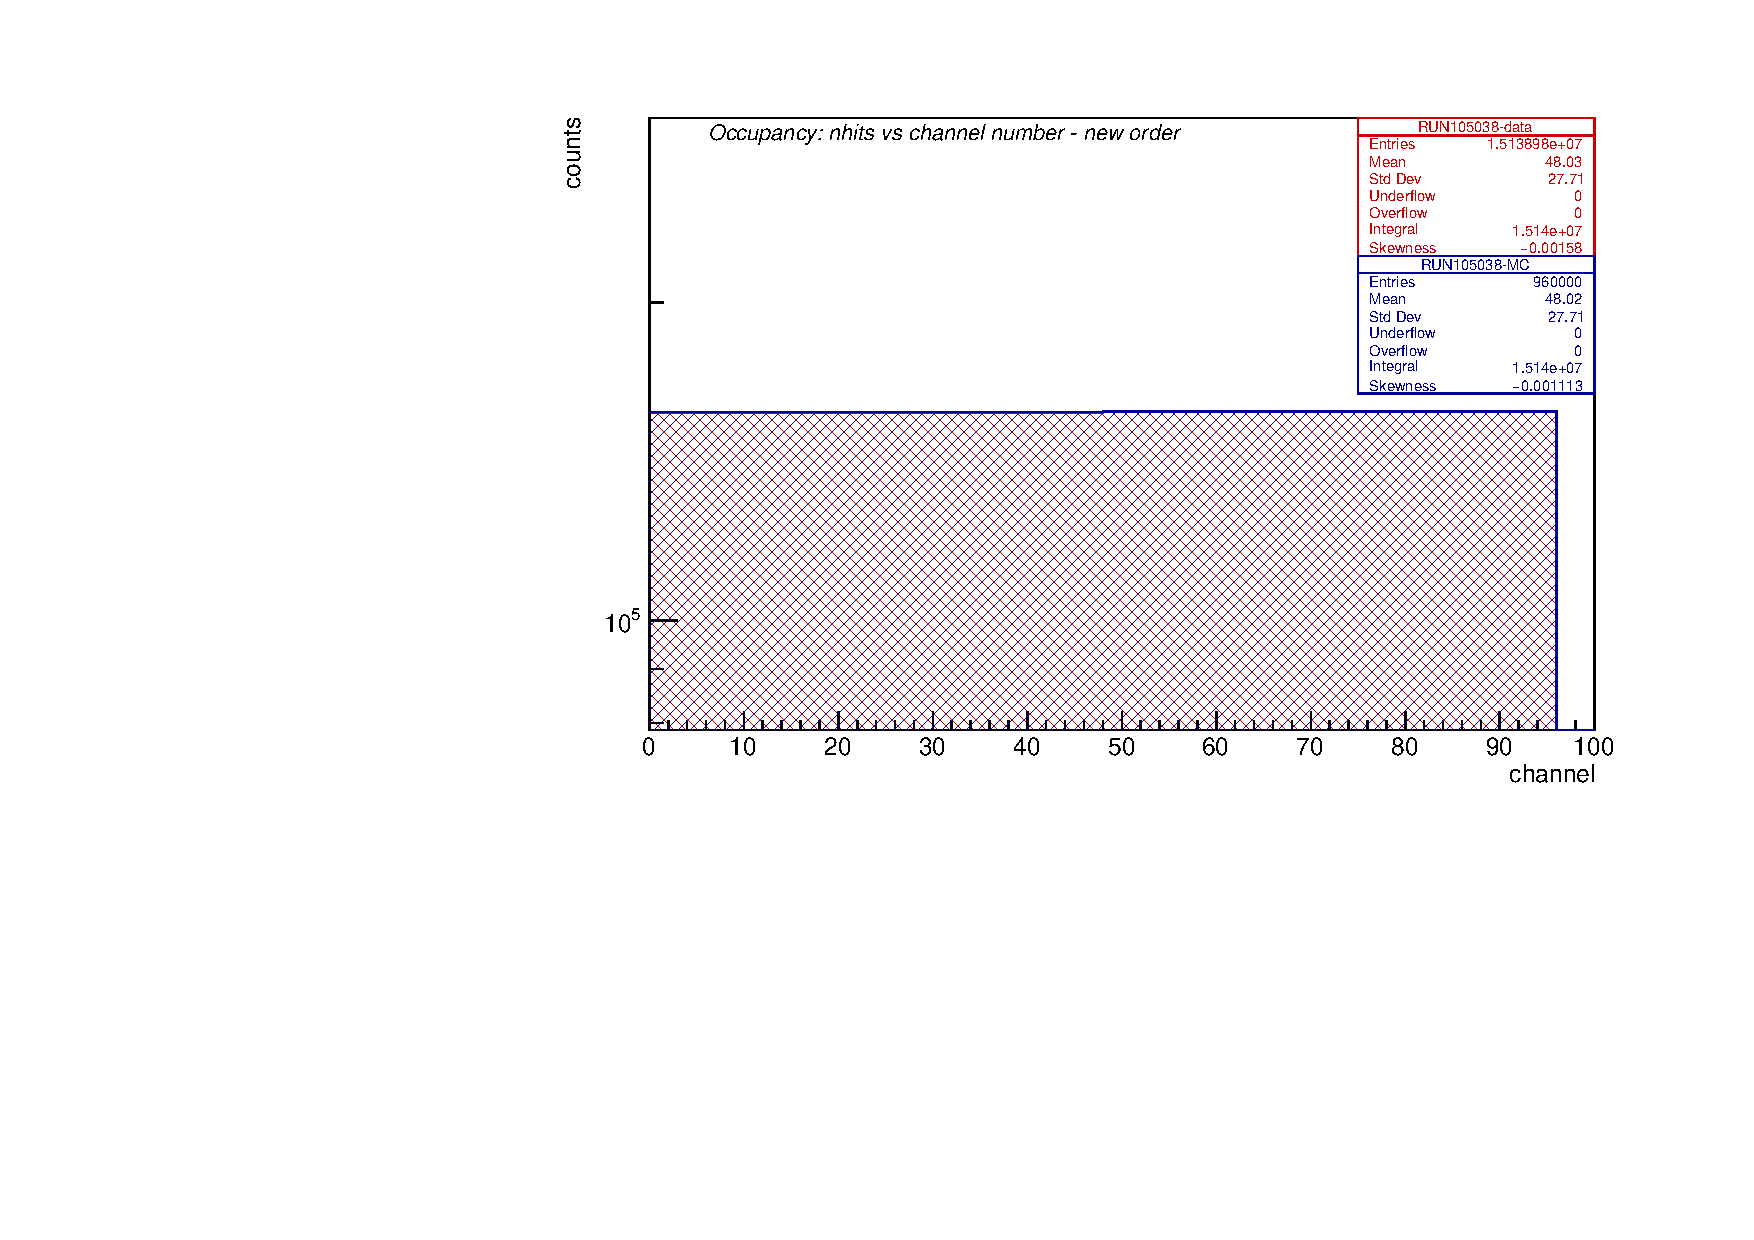
\includegraphics[width =0.8\textwidth]{figures/pdf/figure_00002_nhitsvschannel_roc_simulation_2}
\caption{Occupancy: \add{the} number of hits versus \add{the} channel \add{number} for run 105038.}
\label{fig:5}
\end{figure}


Fig.\ref{fig:67} \add{shows the distribution of the} number of hits in the channel 0 (first FPGA).
\begin{figure}[H]
\centering
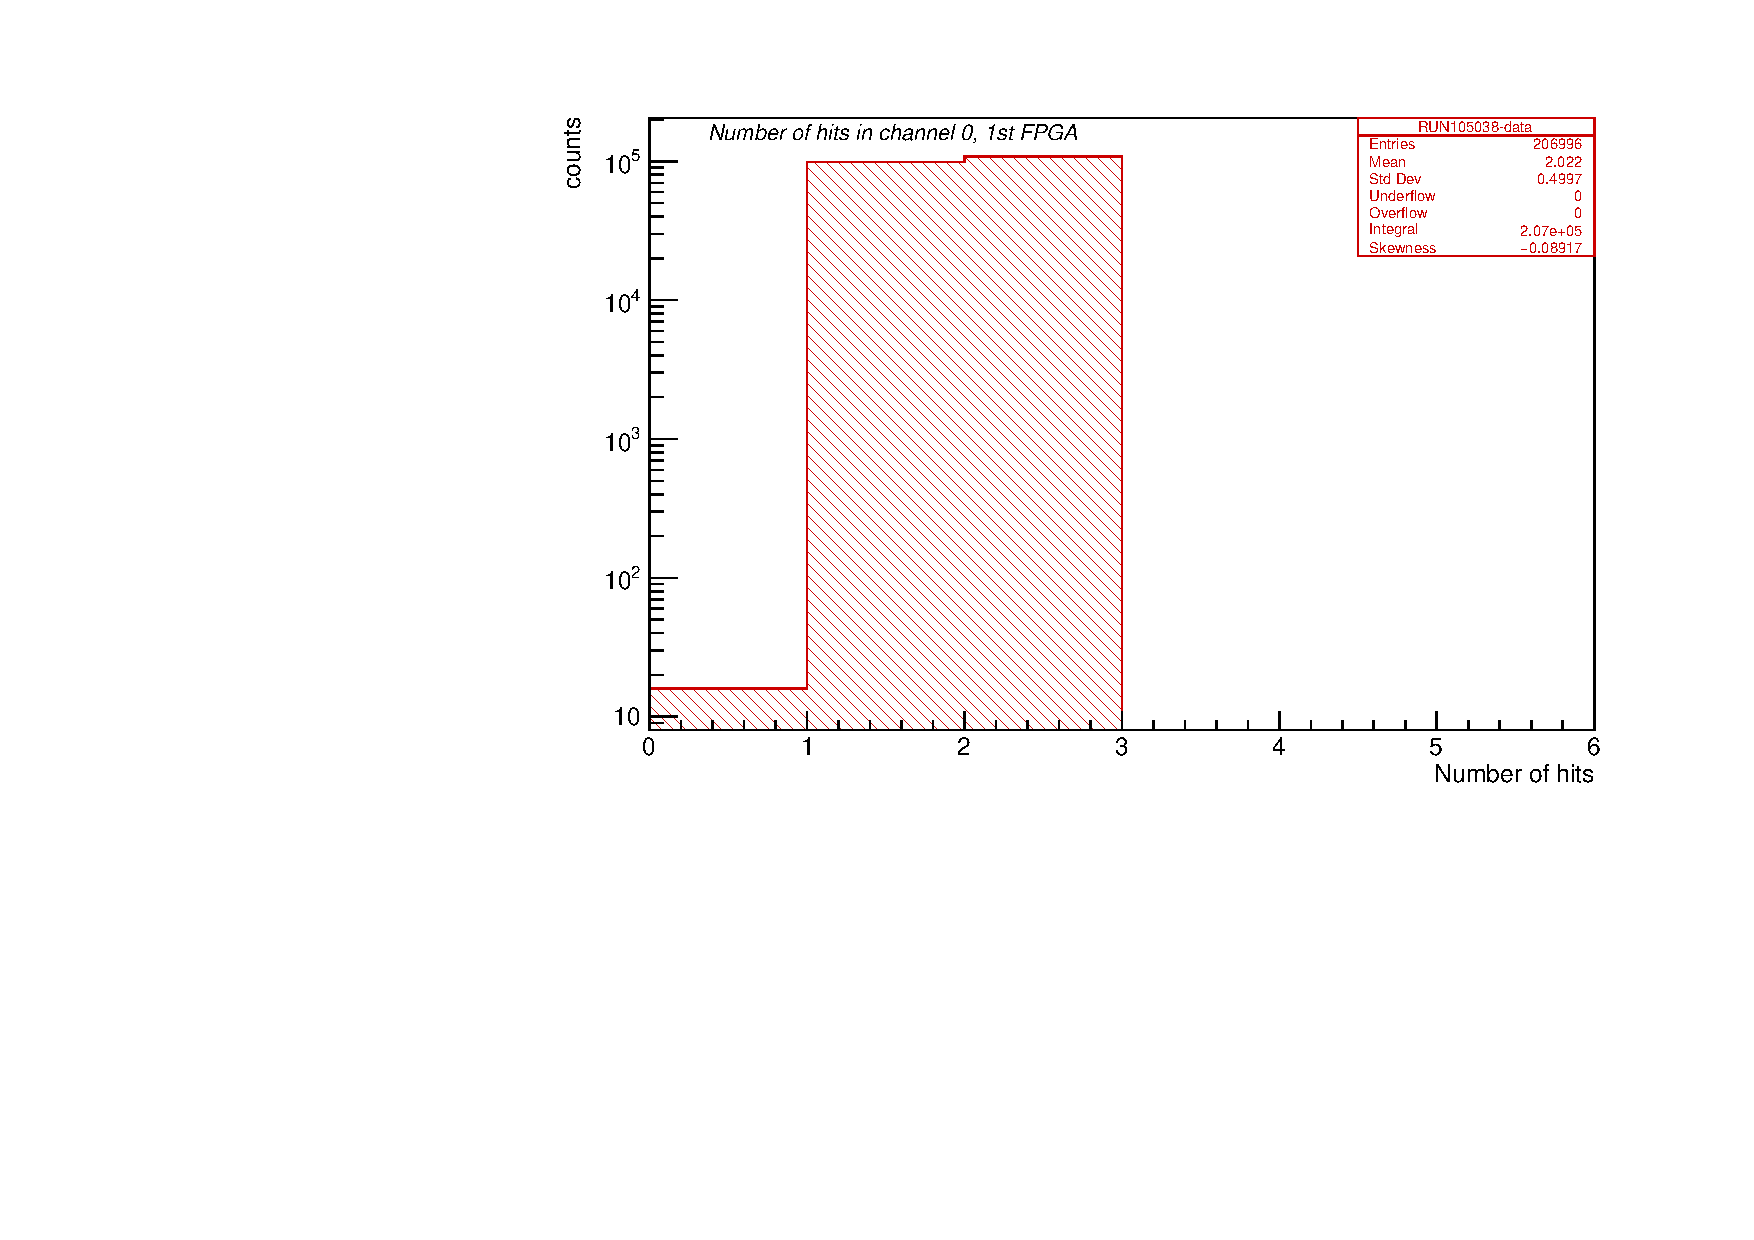
\includegraphics[width =0.8\textwidth]{figures/pdf/figure_00067_nhits_ch00_run105038.pdf}
\caption{
  \del{Number of hits per channel. It is shown that in this configuration
    there could be 0,1 or 2 hits in channel 0, as in other channels.}
  \add{The distribution of the number of hits in channel 0, first FPGA, for run 105038.}
}
\label{fig:67}
\end{figure}

%%%%%%%%%%%%%%%%%%%%%%%%%%%%%%%%%%%%%%%%%%%%%%%%%%%%%%%%%%%%%%%%%%%%%%%%%%%%%%
\subsection{Number of hits}
\del{
  As conclusion we can see in Fig. \ref{fig:6}, the main aspect of non-overflow mode:
the number of hits are not anymore peaked in 255 and so this reflects in the fact
that the number of bytes are not always the same.
}
\add{
  Compared to run 281, the event window in run 105038 was x2 shorter
  and the ROC readout buffer wasn't getting filled up.
  The total number of hits within the event window depends on the relative offset
  of the event window with respect to the FPGA pulsers, and varies from
  144 to 192, as shown in Figure \ref{fig:6}.
}

\begin{figure}[!h]
\centering
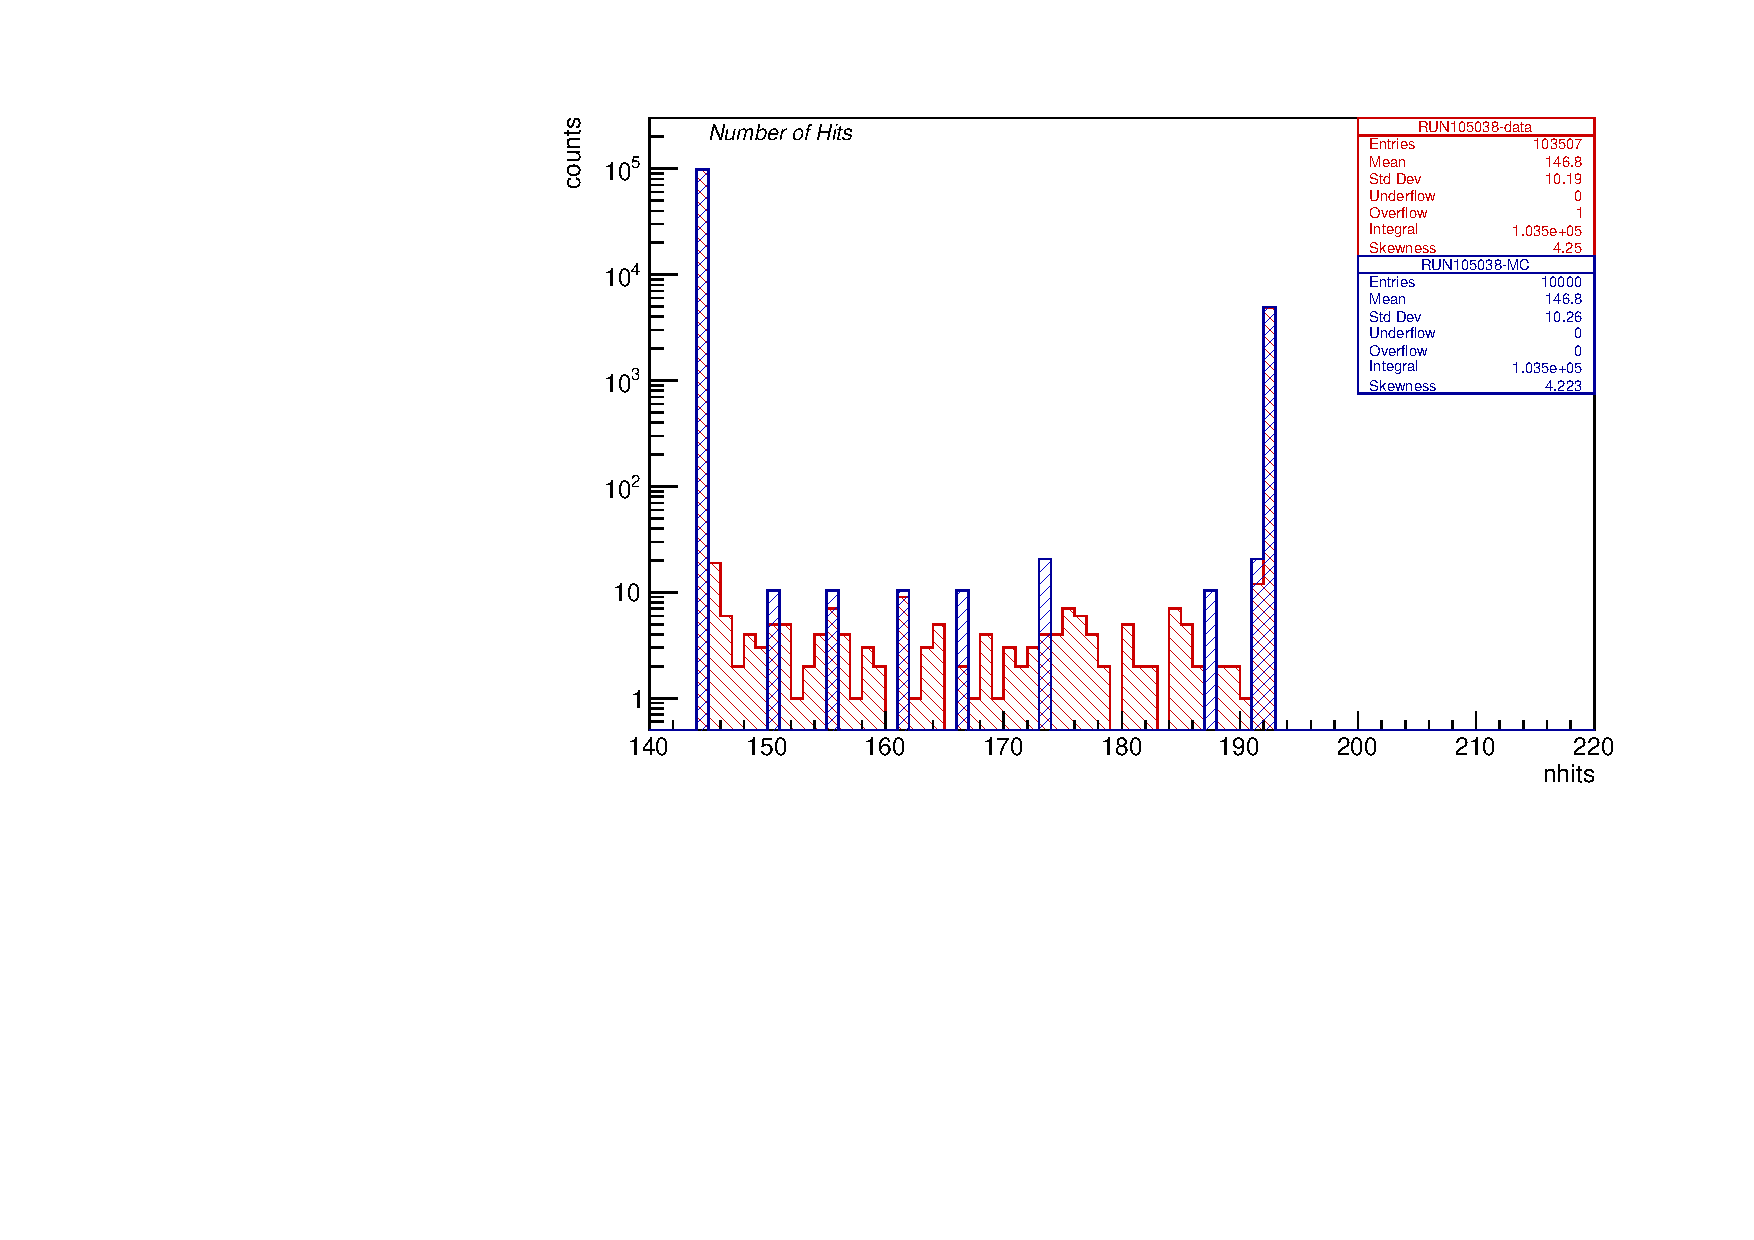
\includegraphics[width =0.8\textwidth]{figures/pdf/figure_00009_nhits_105038}
\caption{
  \del{Total number of hits distribution.}
  \add{Distribution of the total number of hits per event in ``non-saturated'' mode}
}
\label{fig:6}
\end{figure}










%%% Local Variables:
%%% mode: latex
%%% TeX-master: t
%%% End:
